% Lernziele für Lineare Regression
\newcommand{\lernzieleRegression}[1]{
	\begin{itemize}[<+->]
		\item[#1] Ich kann erklären, was eine \textbf{lineare Regression} ist und wofür sie verwendet wird.
		\item[#1] Ich kann den Unterschied zwischen \textbf{unabhängiger} und \textbf{abhängiger} Variable erläutern.
		\item[#1] Ich kann eine \textbf{lineare Funktion} aus zwei Punkten bestimmen.
		\item[#1] Ich kann das Prinzip der \textbf{Kleinste-Quadrate-Methode (OLS)} erklären und anwenden.
		\item[#1] Ich kann eine Regressionsgerade zeichnen und interpretieren.
		\item[#1] Ich kann die \textbf{Qualität einer Regression} anhand von Fehlermassen beurteilen.
		\item[#1] Ich kann eine lineare Regression in \textbf{Python} durchführen.
	\end{itemize}
}

% command to make sure colorboxes don't create whitespace between code lines
% Reduce the space inside colorboxes to avoid extra whitespace between lines
\fboxsep=.6pt

% default settings for listings
\lstset{style=python}

\title[Daten Vorhersagen]{Daten Vorhersagen}

\subtitle{Lineare Regression}

\author[Wendl, Cyril] % (optional)
{Naoki Peter\inst{1} \and Cyril Wendl \inst{2}}

\institute[KZN] % (optional)
{
	\inst{1}%
	Fachschaft Informatik\\
	Kantonsschule Zürich-Nord
	\and
	\inst{2}%
	Fachschaft Informatik\\
	Kantonsschule im Lee
}
\date[\today] % (optional)

\logo{\includegraphics[width=\logosize]{\thelogo}}

\titlegraphic{\vspace{-.7cm}\includegraphics[width=\textwidth]{"Grundlagen_Info/06_Datenbanken/Figures/title-emojis"}}

\frame{\titlepage}


\begin{frame}{Themenübersicht}
	\begin{enumerate}
		\item[\faCheckSquare{}] Daten verstehen (analysieren und visualisieren)
		\item[\faSquare] \textbf{Zahlen vorhersagen}
		\item[\faSquare] Kategorien vorhersagen
	\end{enumerate}
\end{frame}

\begin{frame}{Maschinelles Lernen}
	\begin{figure}[H]
		\only<1->{\centering
\includegraphics[width=0.26\pagewidth]{"Grundlagen_Info/10_Aus_Daten_Lernen/Figures/intro_spam.jpg"}}
		\only<2->{\centering
\includegraphics[width=0.26\pagewidth]{"Grundlagen_Info/10_Aus_Daten_Lernen/Figures/intro_YT.jpg"}}
		\only<3->{\centering
\includegraphics[width=0.26\pagewidth]{"Grundlagen_Info/10_Aus_Daten_Lernen/Figures/intro_scan.jpg"}}
		% \only<4->{\centering
\includegraphics[width=0.3\pagewidth]{"Grundlagen_Info/10_Aus_Daten_Lernen/Figures/intro_recommendation.jpg"}}
	\end{figure}
\end{frame}

\begin{frame}[fragile]{Lernziele}
	\lernzieleRegression{\faSquare}
\end{frame}

\begin{frame}{Zahlen vorhersagen mit Regression}{Unabhängige und abhängige Variablen}
	\begin{table}
		\centering
		\begin{tabular}{rcl}
			\only<1->{\textbf{Unabhängige Variable}} & \only<1->{\phantom{$\rightarrow$}} & \only<1->{\textbf{Abhängige Variable}} \\ \midrule\midrule
			\only<2->{Lernzeit}                      & \only<2->{$\rightarrow$}           & \only<2->{Note in der Prüfung}         \\ \midrule
			\only<3->{Alter eines Autos}             & \only<3->{$\rightarrow$}           & \only<3->{Wiederverkaufswert}          \\ \midrule
			\only<4->{Anzahl Schritte pro Tag}       & \only<4->{$\rightarrow$}           & \only<4->{Kalorienverbrauch}           \\ \midrule
			\only<5->{Aussentemperatur}              & \only<5->{$\rightarrow$}           & \only<5->{Eisverkaufszahlen}           \\ \midrule
			\only<6->{Anzahl Likes auf Social Media} & \only<6->{$\rightarrow$}           & \only<6->{Reichweite eines Posts}      \\
		\end{tabular}
	\end{table}
\end{frame}

\begin{frame}{\textbf{Unabhängige} und \textbf{abhängige Variablen}}
	\begin{table}
		\centering
		\begin{tabular}{p{3cm}|p{5cm}}
			\textbf{Unabhängige Variable} & Kontrollierbare Grösse, beeinflusst andere Variable(n).               \\ \midrule
			\textbf{Abhängige Variable}   & Messbare Grösse, wird beeinflusst von \textit{unabhängiger} Variable. \\
		\end{tabular}
	\end{table}
\end{frame}

\begin{frame}{Zahlen vorhersagen mit Regression}{Unabhängige und abhängige Variablen}
	\begin{columns}
		\column{0.7\textwidth}
		\begin{figure}[H]
			\centering
			
\includegraphics[width=\textwidth]{"Grundlagen_Info/10_Aus_Daten_Lernen/Figures/schlafdauer_vs_note.pdf"}
		\end{figure}
		\column{0.3\textwidth}
		\begin{itemize}[<+->]
			\item \textbf{Unabhängige Variable}: Schlafdauer
			\item \textbf{Abhängige Variable}: Note
			\item \textbf{Ziel}: Vorhersage der Note anhand der Schlafdauer
			\item \textbf{Beispiel}: 7.9 Stunden Schlaf $\rightarrow$ Note 5.5?
		\end{itemize}
	\end{columns}
\end{frame}

\begin{frame}{Lineare Funktion}
	\begin{columns}
		\column{0.7\textwidth}
		\only<1>{
			\begin{figure}[H]
				\centering
				
\includegraphics[width=\textwidth]{"Grundlagen_Info/10_Aus_Daten_Lernen/Figures/schlafdauer_vs_note.pdf"}
			\end{figure}
		}
		\only<2>{
			\begin{figure}[H]
				\centering
				
\includegraphics[width=\textwidth]{"Grundlagen_Info/10_Aus_Daten_Lernen/Figures/schlafdauer_vs_note_2p_reg.pdf"}
			\end{figure}
		}
		\column{0.3\textwidth}
		Einfache Idee: zwei Datenpunkte verbinden, um eine Gerade zu berechnen:
		\begin{table}[H]
			\centering
			\begin{tabular}{p{1.2cm}p{1cm}}
				\toprule
				\textbf{Schlafdauer\newline(=x)} & \textbf{Note \newline(=y)} \\
				\midrule
				3.54                             & 3.57                       \\
				9.617                            & 6.0                        \\
				\bottomrule
			\end{tabular}
		\end{table}

		\begin{equation*}
			\begin{aligned}
				m & = \frac{y_2 - y_1}{x_2 - x_1} \\
				q & = y_1 - m \cdot x_1
			\end{aligned}
		\end{equation*}
	\end{columns}
\end{frame}

\begin{frame}{Qualität der Gerade}
	\begin{columns}
		\column{0.7\textwidth}
		\begin{figure}[H]
			\centering
			
\includegraphics[width=\textwidth]{"Grundlagen_Info/10_Aus_Daten_Lernen/Figures/schlafdauer_vs_note_2p_reg_pred.pdf"}
		\end{figure}
		\column{0.3\textwidth}
		\begin{table}
			\scriptsize
			\setlength{\tabcolsep}{2pt}
			\centering
			\begin{tabular}{c|ccc}
				\toprule
				       & $P_1$ & $P_2$ & $P_3$ \\
				\midrule
				Schlaf & 3.5   & 7.9   & 9.6   \\
				Note   & 3.6   & 6.0   & 6.0   \\
				Vorh.  & 3.6   & 5.3   & 6.0   \\
				Diff.  & 0.0   & -0.7  & 0.0   \\
				\bottomrule
			\end{tabular}
		\end{table}
		\small
		\textbf{Fehler}:
		$$0^2+(-0.7)^2+0^2= \underline{0.5}$$
	\end{columns}
\end{frame}

\begin{frame}{Lineare Regression mit \textbf{OLS} - Ordinary Least Squares (Kleinste Quadrate)}
	$$m = \frac{n\sum x_iy_i - \sum x_i \sum y_i}{n\sum x_i^2 - (\sum x_i)^2}$$
	Das berechnete $m$ ist die Steigung der Geraden, die den Fehler minimiert. Diese kann nun in die Gleichung für $q$ eingesetzt werden:
	$$q = \frac{\sum y_i - m\sum x_i}{n}$$
\end{frame}

\begin{frame}{OLS-Regressionslinie}
	\begin{figure}[H]
		\centering
		
\includegraphics[width=.8\pagewidth]{"Grundlagen_Info/10_Aus_Daten_Lernen/Figures/schlafdauer_vs_note_ols.pdf"}
	\end{figure}
\end{frame}

\begin{frame}{Multiple lineare Regression}
	Manchmal hängt die Vorhersage nicht nur von einer Variable ab\dots
	\begin{itemize}[<+->]
		\item Erfolgreicher Opernsänger \emoji{microphone}
		      \begin{itemize}
			      \item Schönes Aussehen \emoji{sunglasses}
			      \item Gute Stimme \emoji{musical-notes}
		      \end{itemize}
		\item Autokauf \emoji{car}
		      \begin{itemize}
			      \item Preis \emoji{money-bag}
			      \item Marke \emoji{car}
			      \item Baujahr \emoji{calendar}
		      \end{itemize}
	\end{itemize}

\end{frame}

\begin{frame}{Multiple lineare Regression}{Mehrere unabhängige Variablen}
	\begin{columns}
		\column{0.5\textwidth}
		\begin{itemize}
			\item Beispiel: Note über Lernaufwand und Schlaf
			\item Erklärung:
			      \begin{itemize}
				      \item $x_1$: Lernaufwand
				      \item $x_2$: Schlaf
				      \item $y$: Note
			      \end{itemize}
		\end{itemize}
		\begin{block}{Formeln}
			\begin{itemize}[<+->]
				\item Einfache lineare Regression:
				      \[\begin{aligned}
						      y & = \textcolor{red}{q} + \textcolor{blue}{m}x        \\
						        & = \textcolor{red}{a_0} + \textcolor{blue}{a_1} x_1
					      \end{aligned}\]
				\item Multiple lineare Regression:
				      \[\begin{aligned}
						      y = & \textcolor{red}{a_0} + \textcolor{blue}{a_1} x_1 + a_2x_2 + a_3 x_3 \\
						          & + \
						      cdots + a_n x_n
					      \end{aligned}\]
			\end{itemize}
		\end{block}
		\column{0.65\textwidth}
		\begin{figure}[H]
			\centering
			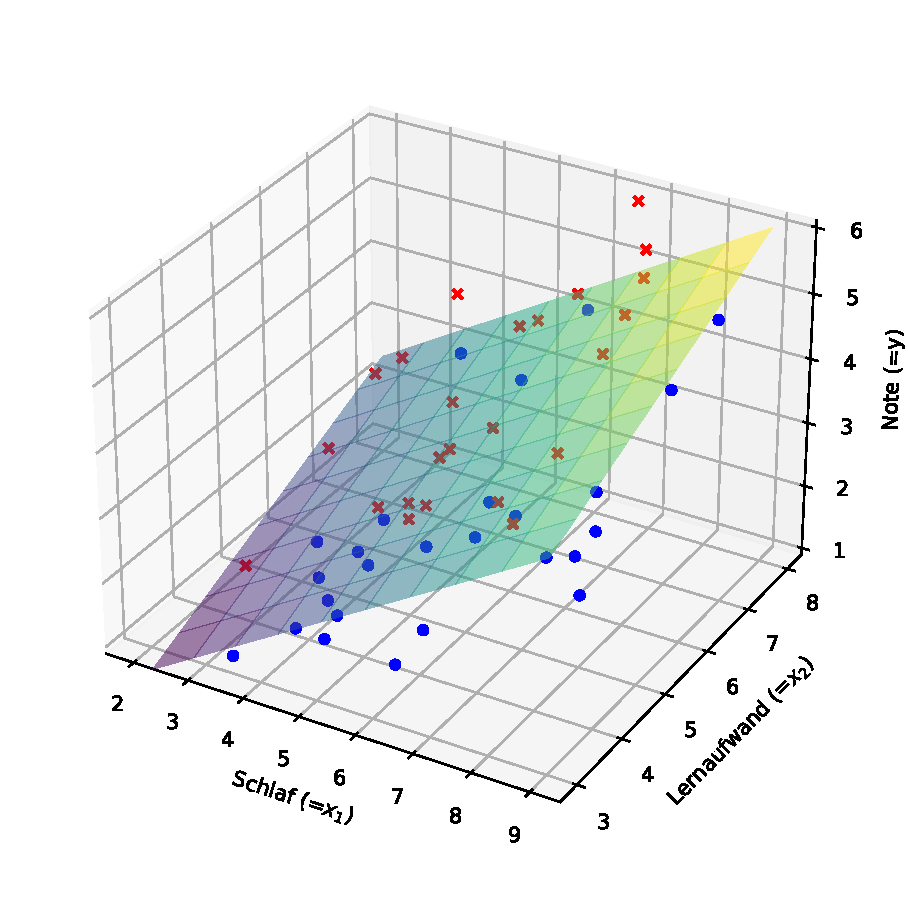
\includegraphics[width=\textwidth]{Grundlagen_Info/10_Aus_Daten_Lernen/Figures/linreg_3d.pdf}
		\end{figure}
	\end{columns}
\end{frame}

\begin{frame}{Auftrag}{Jupyter Notebooks}
	\begin{itemize}
		\item Aufgabenblatt 3a durchlesen und vervollständigen
		\item Aufgabenblatt 3b lösen
	\end{itemize}
\end{frame}



% Lernziele-Frame
\begin{frame}[fragile]{Lernziele}
	\lernzieleRegression{\faCheckSquare}
\end{frame}
